\nte[Section 1.1]{Sep 26 2023 Tue (14:02:35)}{Linear Systems}

\section{Introduction to Linear Systems}
\label{sec:introduction_to_linear_systems}

\begin{definition}[Linear Equation]
  \label{def:linear_equation}

  A \textbf{linear equation} in the variables $x_1, x_2, \dots, x_n$ is an
  equation that can be written in the form $c_1x_1 + c_2x_2 + \dots + c_nx_n =
  k$, where $n \in \R$ and $k, c_1, c_2, \dots, c_n \in \R \cup \C$.
\end{definition}

\begin{example}
  \label{exm:linear_equation}

  Below are some examples of linear equations.

  \begin{multicols}{2}\noindent
    \begin{enumerate}
      \label{enum:linear_equation_1}

      \item $5x_2 + x_3 = 7$
      \item $5x_2 + x_3 = 7$
      \columnbreak
      \item $5x_2 + x_3 = 7$
      \item $5x_2 + x_3 = 7$
    \end{enumerate}
  \end{multicols}

  Here are some equations that aren't linear.

  \begin{multicols}{2}\noindent
    \begin{enumerate}
      \label{enum:non_linear_equation_1}

      \item $\incorrect{x_1 \cdot x_2} = 5 + x_1$.
      \item $\incorrect{\sfrac{x_2}{x_1}} + x_3 = 30$.

      \item $\incorrect{x_2^2} + 8x_3 = x_1$
      \item $\incorrect{\sqrt{x_1}} + x_2 = 120$
    \end{enumerate}
  \end{multicols}
\end{example}

\begin{definition}[System of Linear Equations]
  \label{def:system_of_linear_equations}

  A \textbf{system of linear equations} or \textbf{linear system} is a
  collection of one or more linear equations with them same set of variables
  $x_1, x_2, \dots, x_n$.
\end{definition}

\begin{example}
  \label{exm:system_of_linear_equations}

  Below are some examples of linear systems.

  \begin{multicols}{3}\noindent\centering
    \[%
      \sysdelim..\systeme{
        5x_1 + x_2 = 1,
        -4x_2 + 8x_3 = 2,
        x_1 - 3x_3 = 0
      }
    .\]%
    $3$ equations, $3$ variables\columnbreak
    \columnbreak
    \[%
      \sysdelim..\systeme{
        x_1 + x_2 - 2x_4 = 12,
        4x_3 + 6x_4 = -2,
        2x_1 - x_2 + 9x_3 = 10
      }
    .\]%
    $3$ equations, $4$ variables\columnbreak
    \[%
      \sysdelim..\systeme{
        9x_1 - x_2 = 0,
        7x_1 = 1,
        -6x_2 = 3
      }
    .\]%
    $3$ equations, $2$ variables
  \end{multicols}
\end{example}

\begin{definition}[Solution of Linear System]
  \label{def:solution_of_linear_system}

  A \textbf{solution} of a linear system is a list $\left\{s_1, s_2, \dots,
  s_n\right\}$ of numbers that makes each equation a true statement when the
  values of $s_1, \dots, s_n$ are substituted for $x_1, \dots, x_n$.

  The set of all possible solutions is called the \textbf{solution set} of the
  linear system. Two linear systems are called \textbf{equivalent} if they have
  the same solution set. That is, $\forall x \in S_1, x \in S_2$, where $S_1$
  and $S_2$ are solution sets of two linear systems.
\end{definition}

\begin{example}
  \label{exm:solution_of_linear_system}

  \begin{multicols}{2}
    The list $(5, 6.5,3)$ is a solution to the following linear system
    \[%
      \sysdelim..\systeme{
        2x_1 - x_2 + 1.5x_3 = 8,
        -x_1 + 4x_3 = 7
      }
    ,\]%
    because $2(5) - (6.5) + 1.5(3) \ce 8$ and $-(5) + 4(3) \ce 7$.
    \columnbreak
    \begin{figure}[H]
      \centering

      \begin{tikzpicture}
        \begin{axis}[
          xlabel=$x_1$,
          ylabel=$x_2$,
          xmin=-5.25, xmax=6.25,
          ymin=-3.25, ymax=4.25,
          ]

          \addplot+[domain=-5.25:6.25]{(-1-x)/(-2)} node[below,pos=0.25]{$\ell_1$};
          \addplot+[domain=-5.25:6.25]{(3+x)/(3)} node[above,pos=0.25]{$\ell_2$};
          \addplot[soldot] coordinates{(3,2)};
        \end{axis}
      \end{tikzpicture}

      \caption{}
      \label{fig:two_lines_intersecting_at_a_point}
    \end{figure}
  \end{multicols}
\end{example}

\subsection{Linear System Solutions}
\label{sub_sec:linear_system_solutions}

A linear system has three possible situations.
\begin{enumerate}
  \label{enum:three_possible_solutions}

  \item No solution, making the system \textbf{inconsistent}.
  \item One solution, making the system \textbf{consistent}.
  \item Infinitely many solutions, making the system \textbf{consistent}.
\end{enumerate}

\begin{multicols}{3}\noindent
  \begin{figure}[H]
    \centering

    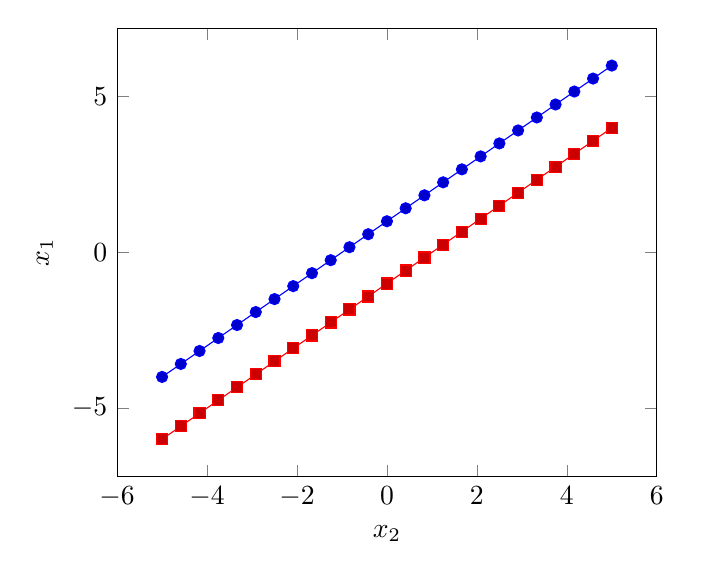
\begin{tikzpicture}
      \begin{axis}[xlabel=$x_2$,ylabel=$x_1$]
        \addplot {x+1};
        \addplot {x-1};
      \end{axis}
    \end{tikzpicture}

    \caption{No solution.}
    \label{fig:no_solution}
  \end{figure}
  \columnbreak
  \begin{figure}[H]
    \centering

    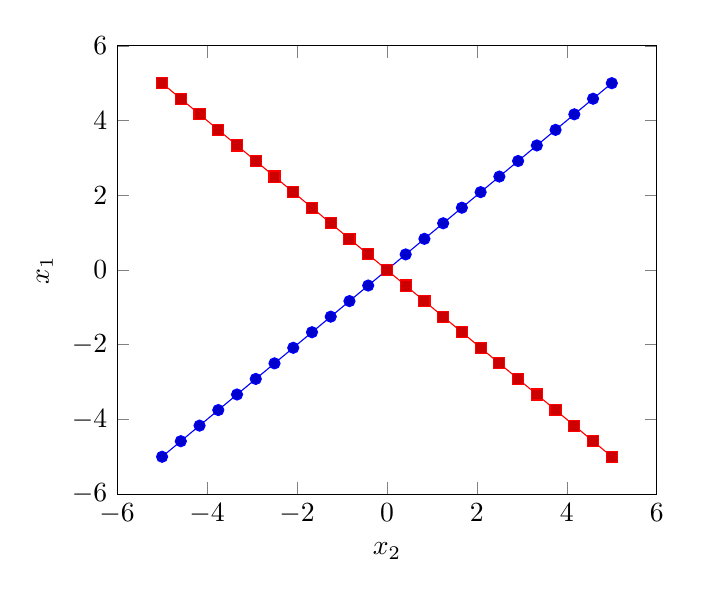
\begin{tikzpicture}
      \begin{axis}[xlabel=$x_2$,ylabel=$x_1$]
        \addplot {x};
        \addplot {-x};
      \end{axis}
    \end{tikzpicture}

    \caption{One solution.}
    \label{fig:on_solution}
  \end{figure}
  \columnbreak
  \begin{figure}[H]
    \centering

    \begin{tikzpicture}
      \begin{axis}[xlabel=$x_2$,ylabel=$x_1$]
        \addplot {x};
        \addplot[style2,dashed] {x};
      \end{axis}
    \end{tikzpicture}

    \caption{Infinite solutions.}
    \label{fig:infinite_solutions}
  \end{figure}
\end{multicols}

% subsection linear_system_solutions (end)

% section introduction_to_linear_systems (end)

\section{Basic Algebra Review}
\label{sec:basic_algebra_review}

Let's consider the following linear system
\[%
  \sysdelim..\systeme{
    2x_1 - 3x_2 = 1,
    6x_1 - 8x_2 = 5
  }
.\]%

There are three ways to solve this system.
\begin{enumerate}
  \label{enum:three_ways_to_solve_a_linear_system}

  \item \textbf{Graphically:} Plot the two lines and find the intersection
    point.

  \item \textbf{Substitution:} Solve one equation for one variable and
    substitute it into the other equation.

  \item \textbf{Elimination:} Add or subtract the equations to eliminate one
    variable.
\end{enumerate}

\subsection{Graphical Method}
\label{sub_sec:graphical_method}

This is the simplest of the three. You plot the two lines and find the
intersection point. The intersection point is the solution to the linear system.

\begin{figure}[H]
  \centering

  \begin{tikzpicture}
    \begin{axis}[
      xlabel={$x_1$},
      ylabel={$x_2$},
      xmin=0, xmax=5,
      ymin=0, ymax=5,
      ]

      \addplot[style1] {(2/3)*x-1/3};
      \addplot[style1] {(3/4)*x-5/8};

      \addplot[soldot] coordinates {(3.5,2)} node[above left] {$\color{black}(\sfrac{7}{2}, 2)$};
    \end{axis}
  \end{tikzpicture}

  \caption{Graphical representation of the system of equations.}
  \label{fig:graphical_representation_of_the_system_of_equations}
\end{figure}

% subsection graphical_method (end)

\subsection{Substitution Method}
\label{sub_sec:substitution_method}

You simply solve for one of the variables, if possible, and then use that to
solve for the other variable. You pick one of the equations, solve for one
variable, and then substitute that into the other equation.
\begin{align*}
  \sysdelim..\systeme{
    2x_1 - 3x_2 = 1,
    6x_1 - 8x_2 = 5
  } &\implies x_1 = \frac{1 + 3x_2}{2} \\
    &\implies \cancel{6}\left(\frac{1 + 3x_2}{\cancel{2}}\right) - 8x_2 = 5 \\
    &\implies 3\left(1 + 3x_2\right) - 8x_2 = 5 \\
    &\implies 3 + 9x_2 - 8x_2 = 5 \\
    &\implies 3 + x_2 = 5 \\
    &\implies x_2 = 2
.\end{align*}
Now that we have $x_2$, we can substitute it into the first equation to find
$x_1$.
\begin{align*}
  2x_1 - 3(2) &= 1 \\
  2x_1 - 6 &= 1 \\
  2x_1 &= 7 \\
  x_1 &= \frac{7}{2}
.\end{align*}

Our solution is $(\sfrac{7}{2}, 2)$, which is what we got from the graphical
method, which checks out.

% subsection substitution_method (end)

\subsection{Elimination Method}
\label{sub_sec:elimination_method}

You have to multiply one of the equations by a constant so that when you add the
two equations together, one of the variables is eliminated.

\begin{center}
  \begin{tabular}{crcccl}
      & $-3\,(~2x_1$ & $-$ & $3x_2$ & $=$ & $1~)$ \\
    $+$ & $6x_1$ & $-$ & $8x_2$ & $=$ & $5$ \\
    \hline
        & $0x_1$ & $+$ & $1x_2$ & $=$ & $2$
  \end{tabular}\quad\quad
  \begin{tabular}{cr}
      & $-3\,\cdot\,[\text{equation 1}]$ \\
    $+$ & $[\text{equation 2}]$ \\
    \hline
        & $[\text{new equation 2}]$
  \end{tabular} \\\vspace{3ex}
  \begin{tabular}{crcccl}
      & $2x_1$ & $-$ & $3x_2$ & $=$ & $1$ \\
    $+$ & $3\,(~0x_1$ & $+$ & $x_2$ & $=$ & $2~)$ \\
    \hline
        & $2x_1$ & $+$ & $0x_2$ & $=$ & $7$
  \end{tabular}\quad\quad
  \begin{tabular}{cr}
      & $[\text{equation 1}]$ \\
    $+$ & $3\,\cdot\,[\text{equation 2}]$ \\
    \hline
        & $[\text{new equation 1}]$
  \end{tabular}
\end{center}

This gives us the new linear system
\[%
  \sysdelim..\systeme{
    0x_1 + 1x_2 = 2,
    2x_1 + 0x_2 = 7
  }
.\]%

We can see that $x_2 = 2$ from the first equation. We can solve for $x_1$ by
dividing both sides by $2$, which gives us $x_1 = \sfrac{7}{2}$, giving us the
solution $(\sfrac{7}{2}, 2)$, just like before.

% subsection elimination_method (end)

% section basic_algebra_review (end)

\section{Introduction to Matrices}
\label{sec:introduction_to_matrices}

\begin{definition}[Matrix]
  \label{def:matrix}

  An $m \times n$ matrix is a rectangular array of numbers with $m$ rows and $n$
  columns. A linear system whose coefficients are aligned by column to form a
  matrix is called its \textbf{coefficient matrix}. The \textbf{augmented
  matrix} of a linear system is its coefficient matrix with an extra last column
  composed of its constants.
\end{definition}

\begin{example}
  \label{exm:coefficient_and_augmented_matrices}

  Below is an example of a linear system with its corresponding coefficient and
  augmented matrix.
  \[%
    \sysdelim..\systeme{
      x_1 - 2x_2 + x_3 = 0,
      2x_2 - 8x_3 = 8,
      5x_1 - 5x_3 = 10
    }~\longleftrightarrow~
    \underset{\text{\small coefficient matrix}}{
      \begin{bNiceMatrix}[r,columns-width=auto,first-row]
        \imp{x_1} & \imp{x_2} & \imp{x_3} \\
        1 & -2 & 1 \\
        0 & 2 & -8 \\
        5 & 0 & -5 \\
      \end{bNiceMatrix}
    }~\longleftrightarrow~
    \underset{\text{\small augmented matrix}}{
      \begin{bNiceArray}{ccc|c}[columns-width=auto,first-row]
        \imp{x_1} & \imp{x_2} & \imp{x_3} &  \\
        1 & -2 & 1 & 0 \\
        0 & 2 & -8 & 8 \\
        5 & 0 & -5 & 10 \\
      \end{bNiceArray}
    }
  .\]%
\end{example}

\begin{notation}
  \label{ntn:augmented_matrices_notation}

  You don't have to always use that bar notation. You can instead use regular
  matrix notation and state if it's an augmented matrix or not. Throughout these
  notes, I'll be using the augmented notation. If you don't see the vertical
  bar, then it's not an augmented matrix.
\end{notation}

\begin{note}
  \label{nte:coefficient_matrix}

  When the variable for the matrix is $A$, then that means the matrix is always
  a coefficient matrix, not an augmented matrix.
\end{note}

\subsection{Uniqueness and Existence Questions}
\label{sub_sec:uniqueness_and_existence_questions}

When encountering a linear system, we generally want to answer two questions
about it:

\begin{purpleframe}[Two Fundamental Questions About a Linear Systems]
  \label{prpl:two_fundamental_questions_about_a_linear_systems} $ $

  \begin{enumerate}
    \label{enum:two_fundamental_questions_for_linear_systems}

    \item \textbf{Existence:} Does the system have any solutions?
    \item \textbf{Uniqueness:} If it does, does it have infinitely many solutions
      or just one?
  \end{enumerate}
\end{purpleframe}

% subsection uniqueness_and_existence_questions (end)

\subsection{Elementary Row Operations}
\label{sub_sec:elementary_row_operations}

\begin{notation}
  For simplicity, I'll use $R_i$ to denote the $i$th row of a matrix. I'll be
  using this notation throughout these notes.
\end{notation}

There are three legitimate row operations you can use when solving linear
systems that keep the solution set the same.
\begin{enumerate}
  \label{enum:elementary_row_operations}

  \item \textbf{Replacement:} Replace on row by the sum of itself and a
    multiple of another row.

    \begin{example}
      \label{exm:replacement}

      Let's replace the second row with the first row multiplied by $2$ and
      added to the second row.
      \[%
        \begin{bNiceArray}{cc|c}[columns-width=auto]
          1 & 2 & 3 \\
          4 & 5 & 6 \\
          7 & 8 & 9 \\
        \end{bNiceArray}
        \quad 2R_1 + R_2 \rightarrow R_2 \longleftrightarrow
        \begin{bNiceArray}{cc|c}[columns-width=auto]
          1 & 2 & 3 \\
          6 & 12 & 18 \\
          7 & 8 & 9 \\
        \end{bNiceArray}
      .\]%
    \end{example}

    \begin{note}
      \label{nte:replacement}

      You can't do something like this: $2R_1 + \incorrect{R_2} \rightarrow
      \incorrect{R_1}$. When you do that, you might change the solution to the
      linear system.
    \end{note}

  \item \textbf{Interchange:} Interchange two rows.

    \begin{example}
      \label{exm:interchange}

      Let's interchange the first and second rows
      \[%
        \begin{bNiceArray}{cc|c}[columns-width=auto]
          1 & 2 & 3 \\
          4 & 5 & 6 \\
          7 & 8 & 9 \\
        \end{bNiceArray}
        \quad R_1 \rightarrow R_2 \longleftrightarrow
        \begin{bNiceArray}{cc|c}[columns-width=auto]
          4 & 5 & 6 \\
          1 & 2 & 3 \\
          7 & 8 & 9 \\
        \end{bNiceArray}
      .\]%
    \end{example}

  \item \textbf{Scaling:} Multiply all entires in a row by a nonzero constant.

    \begin{example}
      \label{exm:scaling}

      Let's scale the first row by $2$
      \[%
        \begin{bNiceArray}{cc|c}[columns-width=auto]
          1 & 2 & 3 \\
          4 & 5 & 6 \\
          7 & 8 & 9 \\
        \end{bNiceArray}
        \quad 2R_1 \rightarrow R_1 \longleftrightarrow
        \begin{bNiceArray}{cc|c}[columns-width=auto]
          2 & 4 & 6 \\
          4 & 5 & 6 \\
          7 & 8 & 9 \\
        \end{bNiceArray}
      .\]%
    \end{example}
\end{enumerate}

% subsection elementary_row_operations (end)

% section introduction_to_matrices (end)

\section{Solving Linear Systems with Row Operations}
\label{sec:solving_linear_systems_with_row_operations}

Let's re-use the linear system from \cref{sec:basic_algebra_review}
\[%
  \sysdelim..\systeme{
    2x_1 - 3x_2 = 1,
    6x_1 - 8x_2 = 5
  }
.\]%

That linear system becomes the following augmented matrix
\[%
  \begin{bNiceArray}{cc|c}[columns-width=auto]
    2 & -3 & 1 \\
    6 & -8 & 5 \\
  \end{bNiceArray}
.\]%

We can use the three row operations to solve this linear system
\begin{align*}
  \sysdelim..\systeme*{
    -3R_1 + R_2 \rightarrow  R_2
  } &\longleftrightarrow
  \begin{bNiceArray}{cc|c}[columns-width=auto]
    2 & -3 & 1 \\
    0 & 1 & 2 \\
  \end{bNiceArray} \\
  \sysdelim..\systeme*{
    3R_2 + R_1 \rightarrow R_1
  } &\longleftrightarrow
  \begin{bNiceArray}{cc|c}[columns-width=auto]
    2 & 0 & 7 \\
    0 & 1 & 2 \\
  \end{bNiceArray} \\
  \sysdelim..\systeme*{
    \sfrac{1}{2}R_1 \rightarrow  R_1
  } &\longleftrightarrow
  \begin{bNiceArray}{cc|c}[columns-width=auto]
    1 & 0 & \sfrac{7}{2} \\
    0 & 1 & 2 \\
  \end{bNiceArray}
.\end{align*}

This gives us the new linear system
\begin{align*}
  \begin{bNiceArray}{cc|c}[columns-width=auto]
    1 & 0 & \sfrac{7}{2} \\
    0 & 1 & 2
  \end{bNiceArray}
  \longleftrightarrow
  \sysdelim..\systeme{
    1x_1 + 0x_2 = \sfrac{7}{2},
    0x_1 + 1x_2 = 2
  } &\implies x_1 = \frac{7}{2} \\
    &\implies x_2 = 2
.\end{align*}

\begin{note}
  \label{nte:row_operations}

  You may notice that the operations performed on each row is similar to the
  operations we did when we were solving the linear system through elimination
  in \cref{sub_sec:elimination_method}.
\end{note}

% section solving_linear_systems_with_row_operations (end)

\newpage
